\documentclass[12pt,a4paper]{article}
\usepackage{geometry}
\usepackage{listings}
\usepackage{amsmath}
\usepackage{amssymb}
\usepackage{graphicx}
\usepackage{hyperref}
\graphicspath{ {./images/} }
\lstset{
    escapeinside={(*}{*)},
}
\lstdefinestyle{mystyle}{
    basicstyle=\ttfamily\footnotesize,
    breakatwhitespace=false,
    breaklines=true,  
    captionpos=b,
    keepspaces=true,
    numbers=left,
    numbersep=5pt,
    showspaces=false,
    showstringspaces=false,
    showtabs=false,
    tabsize=2
}
\lstset{style=mystyle}
\geometry{
    a4paper,
    left=20mm,
    right=20mm,
    top=20mm,
}

\begin{document}
\section*{Programming Part Report}
\section*{(a)}
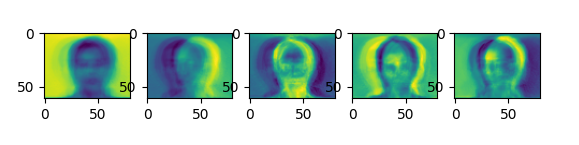
\includegraphics{Figure1.png}
\newpage
\section*{(b)}
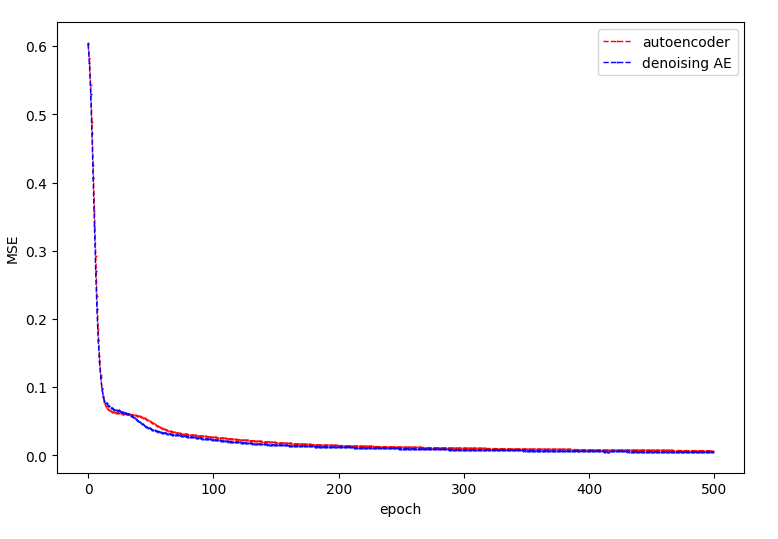
\includegraphics{Figure2.png}
\newpage
\section*{(c)}
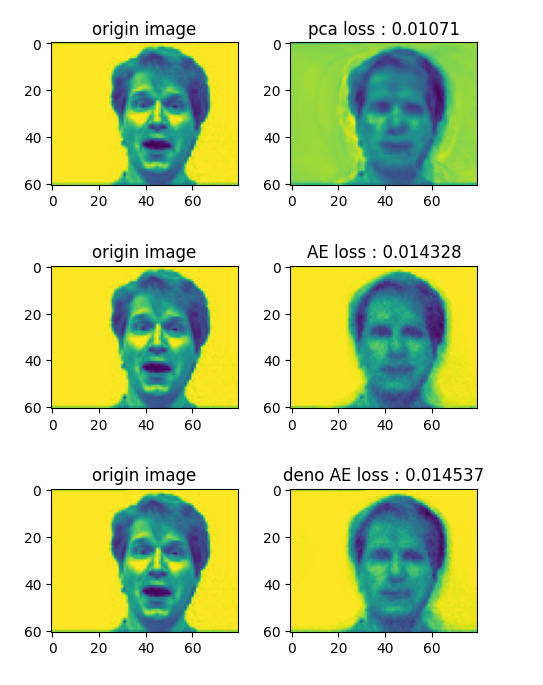
\includegraphics{Figure3.png}
\newpage
\section*{(d)}
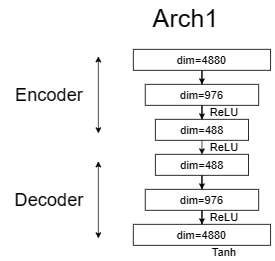
\includegraphics{4-1.png}\\
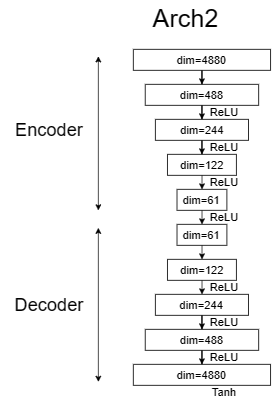
\includegraphics{4-2.png}
\newpage
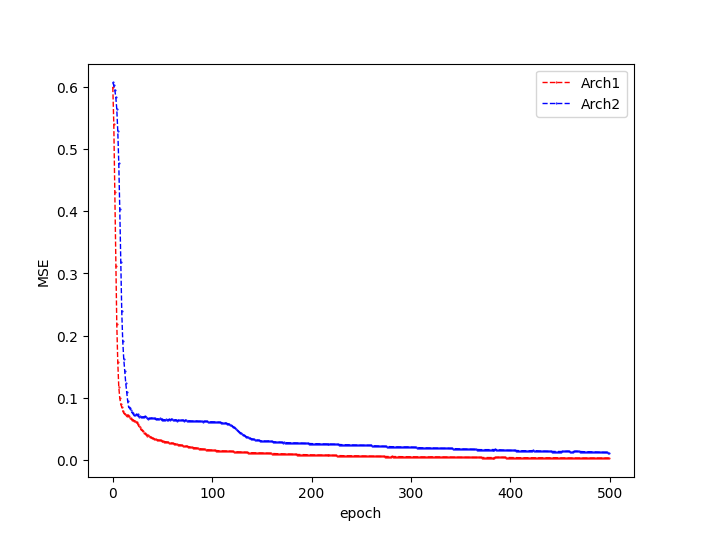
\includegraphics{Figure4.png}
The two architectures are trained under epoch:500, batchSize:45, learning rates:1e-4 and
optimizer:AdamW. Observing the trainning curve, I find the curve of Arch1 is generally smaller than the curve of Arch2, that is,
the MSE loss of Arch1 is smaller than the one of Arch2. Also, when it comes to reconstruction loss, the loss of Arch1 is about 0.01413 while the loss of
Arch2 is about 0.01783. Based on these results, I think a shallow but fatter denoising autoencoder may outperform a deeper but thinner one. This might because
a fatter network can preserve more information when decoding and a deeper network may be more difficult to optimize.
\newpage
\section*{(e)}
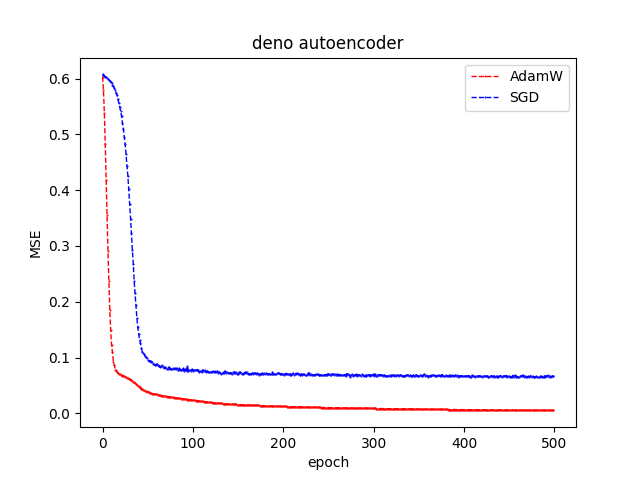
\includegraphics{Figure5.png}\\
I tired two optimizer, one is vanilla SGD and another one is AdamW.
Based on the trainning curve, I find AdamW can converge slightly faster than SGD. 
However, the overall performence of AdamW defeat the one of SGD totally. 
The result may because AdamW can dynamically adjust learning rates and use momentum to improve trainning while vanilla SGD simply train the model.



\end{document}